%%% LyX 2.0.5.1 created this file.  For more info, see http://www.lyx.org/.
%%% Do not edit unless you really know what you are doing.
%\documentclass[twoside,english]{report}
%\usepackage[T1]{fontenc}
%\usepackage[latin9]{inputenc}
%\setcounter{secnumdepth}{3}
%\setcounter{tocdepth}{3}
%\usepackage[active]{srcltx}
%\usepackage{verbatim}
%\usepackage{graphicx}
%\usepackage{setspace}
%\usepackage[numbers]{natbib}
%\doublespacing
%
%\makeatletter
%
%%%%%%%%%%%%%%%%%%%%%%%%%%%%%%% LyX specific LaTeX commands.
%\providecommand{\LyX}{L\kern-.1667em\lower.25em\hbox{Y}\kern-.125emX\@}
%%% Because html converters don't know tabularnewline
%\providecommand{\tabularnewline}{\\}
%
%\makeatother
%
%\usepackage{babel}
%\begin{document}

\chapter{Chapter 1}

This is chapter 1.

\nomenclature{$m$}{The mass of one angel} 



\section{Arabic}
The word Jabal \RL{jbl}

\section{Algorithms}
\begin{algorithm}
$i=0$\;
$sum=0$\;
$FSP = \emptyset $\;
\While{$i<L+1$}
{
	$j = \mathop {\arg \min }\limits_k \left( {D\left( {i,k} \right)} \right)$\;
	$FSP = FSP \cup \left\{ j \right\}$\;
	$sum = sum + D\left( {i,j} \right)$\;
	$i=j$\;
}
\caption{Forward Segmentation Selection (FSS)}
\label{alg:fss}
\end{algorithm}


\section{Figures}
\begin{figure}
\centering
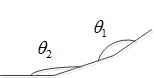
\includegraphics[width=6cm]{./figures/sandbox}       
\caption{The Tunisian city name kambot \RL{kmbw.t}. It contains two word parts (\RL{kmbw} and \RL{.t}). The main body of the first WP is written using three strokes: 1. The letter \RL{k-} 2. The connected letters combination \RL{-mbw} 3. The additional dot of the letter \RL{-b-}. The second WP contains only a single letter (\RL{.t}) and is written using two strokes, the main body and an additional stroke.}
\label{fig:kmbot}
\end{figure}

\begin{figure}[h]
\centering
        \subfloat[]{
            \label{fig:letters_same_body_1}
            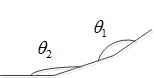
\includegraphics[width=0.3\textwidth]{./figures/sandbox}
        }
        \subfloat[]{
           \label{fig:letters_same_body_2}
           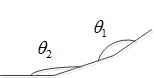
\includegraphics[width=0.3\textwidth]{./figures/sandbox}
        }        
    \caption{Samples of redundant Candidate point at the beginning of the stroke.}
   \label{fig:oversegmentation_begin}
\end{figure}




\begin{comment}
Then in the text you can use Insert citation (use the icon for the
quick use)
\end{comment}



\section{Citations}

The file references.bib in this folder is an example of how to organize
the bibliography database. It is very simple to add a reference/citation
to one of the items in the bibliography list, e.g. see the best source
of information regarding the OpenPTV origins: \citet{Dracos1996}.
Simply use: Insert -> Citation and choose from the list on the left.
Add it to the list on the right and you'll be able to choose the format
of author-year or author-number or just number to the references.
At the same time, at the end of the document you'll find References
chapter with all the cited references automatically chosen and included. 
%\end{document}
